%2146
\newpage
\subsection{\ruby{立体的}{りっ|たい|てき}な絵を出すには}

いままで\ruby{平面的}{へい|めん|てき}な絵を使ってきました。いわゆる「2D」と呼ばれる\ruby{表現}{ひょう|げん}です。

ゲームやCGでは、立体的な「3D」表現が使われています。実際に、立体的な絵を出すプログラムを動かしてみましょう。


先ほどコピーした「/home/ユーザー名/sample」フォルダの中からプログラムを読み込みます。

ファイル→「開く」メニューから「/home/ユーザー名/sample/hgimg4」内の「light\_test3.hsp」を読み込んでください。


\begin{figure}[H]
    \begin{center}
      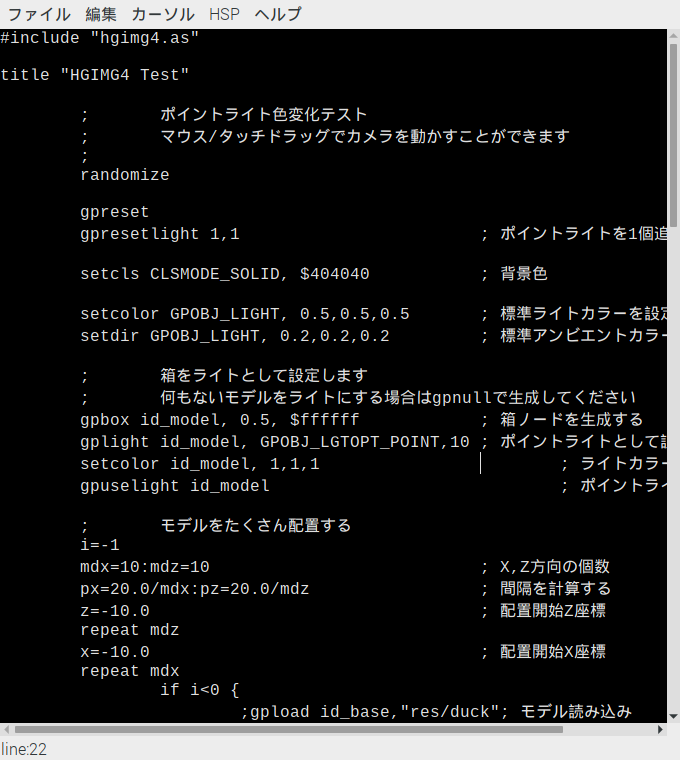
\includegraphics[keepaspectratio,width=10.971cm,height=8.229cm]{text04-img/s_lighttest3s.png}
      \caption{light\_test3s.hspのプログラム}
    \end{center}
    \label{fig:prog_menu}
\end{figure}

[F5]キーで実行すると絵が動きます。

3D表現の画面を出す場合でも、プログラミングの方法は変わりません。ただし、今まで「横」「縦」という2つの\ruby{軸}{じく}があったものが、「横」「縦」「\ruby{奥行}{おく|ゆ}き」という3つの軸に増えて、絵を出す方法も\ruby{複雑}{ふく|ざつ}になります。

\begin{figure}[H]
    \begin{center}
      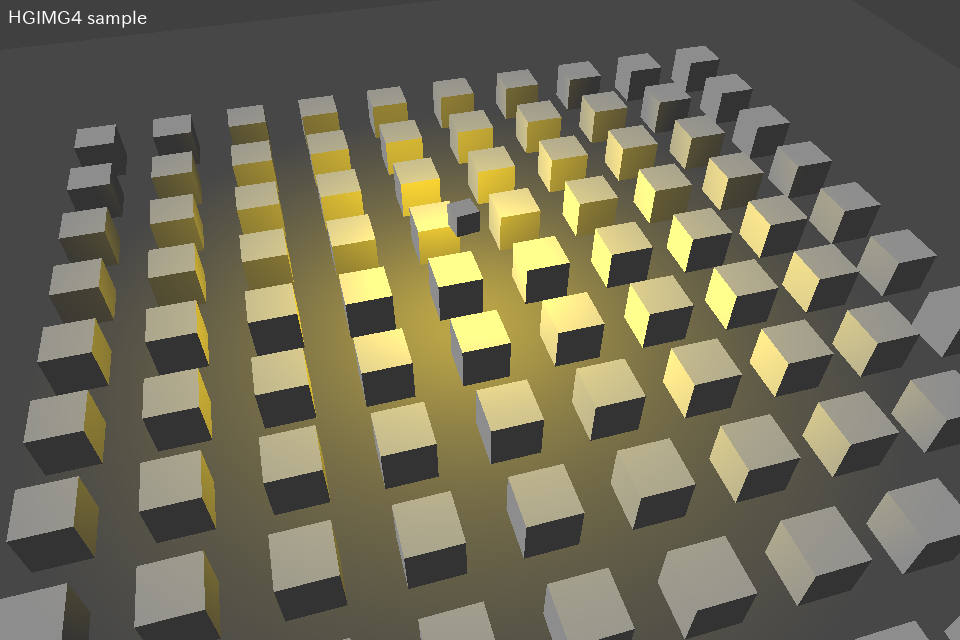
\includegraphics[keepaspectratio,width=10.971cm,height=8.229cm]{text04-img/s_lighttest3.png}
      \caption{light\_test3.hspの実行画面}
    \end{center}
    \label{fig:prog_menu}
\end{figure}


変数や条件判断といった基本的な\ruby{要素}{よう|そ}は変わらないので、まず「2D」のやり方をよく覚えて、さらにそこからステップアップすることをおすすめします。

もう1つ、立体的なキャラクターを出すプログラムを見てみましょう。


ファイル→「開く」メニューから「/home/ユーザー名/sample/pronama3d」内の「pronama2.hsp」を読み込んでください。

[F5]キーで実行するとプロ生ちゃんというキャラクターがダンスする画面になります。


\begin{figure}[H]
    \begin{center}
      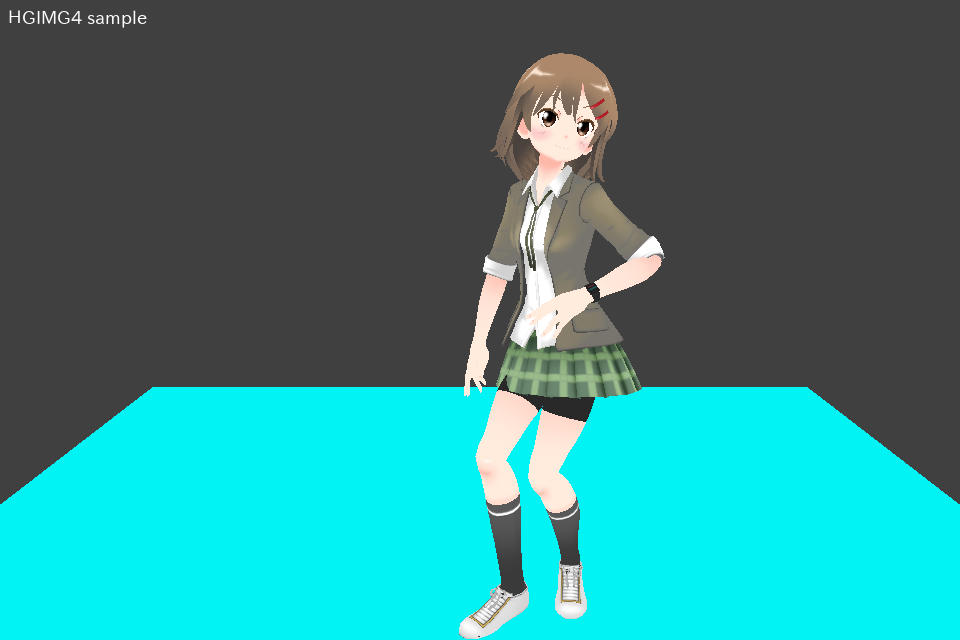
\includegraphics[keepaspectratio,width=10.971cm,height=8.229cm]{text04-img/s_pronama2.png}
      \caption{pronama2.hspの実行画面}
    \end{center}
    \label{fig:prog_menu}
\end{figure}

立体的な絵は、GIMPのような絵を描くツールではなく、3Dグラフィックツールと呼ばれる、形そのものを細かく決めるツールによって作られています。これは、2Dの絵を描くよりもずっと難しい作業です。しかし、仕組みがわかって\ruby{学習}{がく|しゅう}すれば作れるものでもあるのです。


皆さんが使っているラズベリーパイは、スマホやPCと同じような3D表示にも\ruby{対応}{たい|おう}した\ruby{高性能}{こう|せい|のう}なコンピュータです。

応用によって\ruby{本格的}{ほん|かく|てき}なゲームも遊べますし、それを作りだすこともできることを覚えておいてください。


\begin{figure}[H]
    \begin{center}
      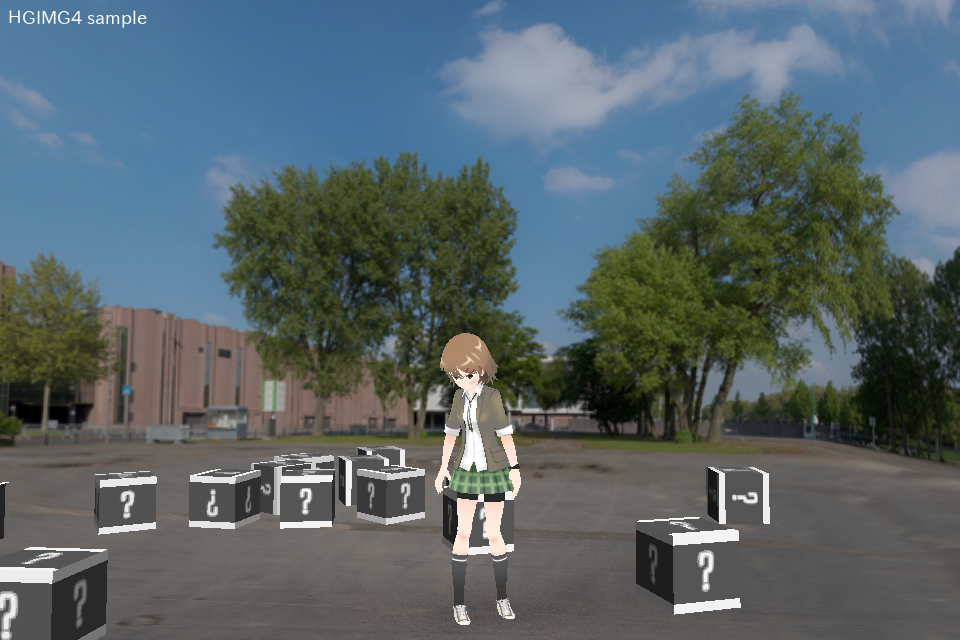
\includegraphics[keepaspectratio,width=10.834cm,height=7.514cm]{text04-img/s_pronamabox.png}
      \caption{背景とキャラクターを同時に出した画面}
    \end{center}
    \label{fig:prog_menu}
\end{figure}

%2250
